% !TeX spellcheck = en_US
% !TeX encoding = utf8
% !TeX program = xelatex
% !BIB program = bibtex

\documentclass[12pt]{article}
	\usepackage{amsmath,amssymb,amsfonts}
	\usepackage{latexsym}
	\usepackage{graphicx}
	\usepackage{verbatim}
	\usepackage{booktabs}
	\usepackage[usenames,dvipsnames,svgnames,table]{xcolor}
	\usepackage{todonotes} % Required for the boxes that questions appear in
	\usepackage{mmstyles}
	
	\newcommand{\mybox}[1]
	{
	\par\noindent
	\todo[inline, backgroundcolor=SkyBlue!40,bordercolor=SkyBlue,size=\large]{\textbf{#1}}
	
	}
	
	\usepackage[top=25mm, bottom=25mm, left=18mm, right=18mm]{geometry}

	\usepackage{fancyhdr}
	\pagestyle{fancy}
	\lhead{Linear Optimization Assignment \#1}
	\chead{}
	\rhead{Due: Sunday, April 15, 23:59:59}
	\renewcommand{\headrulewidth}{0.3pt}

	% \usepackage[framed,numbered,autolinebreaks,useliterate,final]{mcode}
	\usepackage{listings}
	\title{\textbf{Linear Optimization Assignment \#2}}
	\author{Due: Sunday, April 15, 23:59:59}
	\date{}

	\makeatletter
	\def\@seccntformat#1{%
		\expandafter\ifx\csname c@#1\endcsname\c@section\else
		\csname the#1\endcsname\quad
		\fi}
	\makeatother

	\usepackage{multirow}

	\usepackage{sectsty}
	% \sectionfont{\color{NavyBlue}\selectfont}
	% \subsectionfont{\color{SkyBlue}\itshape\selectfont}

	\newcommand{\abs}[1]{\left| #1 \right| }
	\newcommand{\norm}[1]{\left\| {#1} \right\|}
	% \let\oldsection\section
	% \renewcommand\section{\newpage\oldsection}

	\usepackage{titlesec,titletoc} 
	\renewcommand*{\thesection}{\color{NavyBlue}Problem \arabic{section}:} 
	\titleformat{\section}[hang]{\bfseries}{\thesection}{1em}{}{}

	\renewcommand*{\thesubsection}{\color{SkyBlue}Solution \arabic{section}.\arabic{subsection}:} 
	\titleformat{\subsection}[hang]{\itshape}{\thesubsection}{1em}{}{}
	\newcommand{\red}[1]{{\color{red}{#1}}}
	% \setlength{\parsep}{0em}
	\setlength{\parskip}{.33em}
	\setlength{\parindent}{0em}	

	\providecommand{\tightlist}{%
	\setlength{\itemsep}{0pt}\setlength{\parskip}{0pt}}
  
\begin{document}
% \vspace{-1em}
\maketitle

\textbf{\color{NavyBlue}Instruction:} Write a report and complete code.
Download the code from ftp(10.13.71.168). Upload them to ftp(10.13.72.84).
\begin{itemize}
	\tightlist
	\item Upload:
	      \begin{itemize}
		      \tightlist
		      \item    Address: 10.13.72.84
		      \item Username: opt; Passwd:  opt18; Port: 21
	      \end{itemize}
	\item Download:
	      \begin{itemize}
		      \tightlist
		      \item Address: 10.13.71.168
		      \item  Username: opt; Passwd:  opt18; Port: 21
	      \end{itemize}
\end{itemize}


% \begin{abstract}
% 	Enter a short summary here. What topic do you want to investigate and why? What experiment did you perform? What were your main results and conclusion?
% \end{abstract}

\section{MP Neuron}

A McCulloch-Pitts (M-P) neuron accepts bipolar input $x_i \in \{-1,1\}$ and gives  $y=\mathrm{sgn} (\sum_{i=1}^{m} w_ix_i + b) $.

Give weights and bias for a M-P neuron with inputs
$x,y,z \in \{-1,1\}$ and whose output is  $z$ if $x = -1$ and $y = 1$, and is $-1$ otherwise.

\subsection{MP Neuron}

\begin{center}
	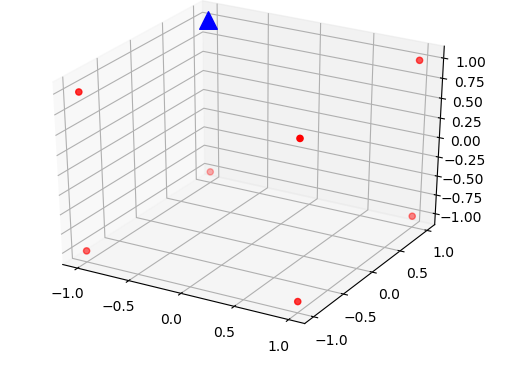
\includegraphics[width=.5\textwidth]{fig/2018-04-02-14-19-18.png}
\end{center}

All separating hyperplanes are correct, \eg, $-x+y+z-2=0$, $f(x,y,z)=\mathrm{sgn}(-x+y+z-2)$.

% \section{Problem 2.}
% The following figure shows the decision regions of four classes. Design a
% classifier for these linearly inseparable classes, using a network consists of M-P neurons with
% three output units. For class $i$ $(1 \le i \le 3)$, classification requires that $y_i = 1$, with $y_j = -1$ for
% $j \ne i$. Class 4 is recognized when $y_i = -1$ for $1 \le i \le 3$.

% \begin{figure}[!htbp]
% 	\centering
% 	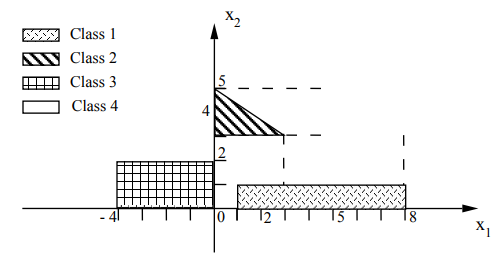
\includegraphics[width=0.7\textwidth]{fig/2018-03-17-14-09-07.png}
% \end{figure}

% ----------------------------------------------------------------------------------------
\newpage 
\section{Gradient Descent}
SGD has trouble navigating ravines, i.e. areas where the surface curves much more steeply in one dimension than in another, which are common around local optima. Momentum is a method that helps accelerate SGD in the relevant direction and dampens oscillations as can be seen in fig~\ref{fig:momentum}.

\begin{eqnarray}
	v_t & = & \mu v_{t-1} + \varepsilon \nabla_u f(u) \label{eq:1} \\
	u_{t+1} & =& u_{t} - v_t \label{eq:2}
\end{eqnarray}

\begin{figure}[!htbp]
	\centering
	
\includegraphics[width=.7\textwidth]{fig/2018-03-19-13-38-08.png}
	\caption{Left: SGD without momentum; Right: SGD with momentum} \label{fig:momentum}
\end{figure}

\begin{description}
	\item[a).] Execute four iterations of gradient descent with momentum to find the minimum of
	      the function $f(u) = \frac{u^3}{3} + 50 u^2-100u-30$. Start with $u_0 = 20$ and $v_0=0$, use a learning rate
	      that is set to $\varepsilon = 0.01$, and parameter $\mu$ set to $0.1$.
	\item[b).] Evaluate the benefit of using a momentum for the task in a). by comparing your
	      findings to the vanilla gradient descent method.
\end{description}

\subsection{Gradient Descent}

Strictly follow formula \ref{eq:1} and \ref{eq:2}.

\begin{itemize}
	\tightlist
	\item $u_1=20, v_1=23$
	\item $u_2=-3, v_1=-1.61$
	\item $u_3=-1.39, v_3\approx -2.53$
	\item $u_4=1.14,v_4=-0.099$
\end{itemize}

Momentum aims primarily to solve two problems: poor conditioning of the Hessian matrix and variance in the stochastic gradient. In fig \ref{fig:momentum}, we illustrate how momentum overcomes the first of these two problems. The contour lines depict a quadratic loss function with a poorly conditioned Hessian matrix.  At each step along the way, we draw an arrow indicating the step that gradient descent would take at that point. We can see that a poorly conditioned quadratic objective looks like a long, narrow valley or canyon with steep sides. Momentum correctly traverses the canyon lengthwise, while gradient steps waste time moving back and forth across the narrow axis of the canyon.

% ----------------------------------------------------------------------------------------
\newpage 
\section{Forward-Backward-Pass}
Examine the multi-layer perceptron given in fig~\ref{fig:mlp}.

\begin{figure}[!htbp]
	\centering
	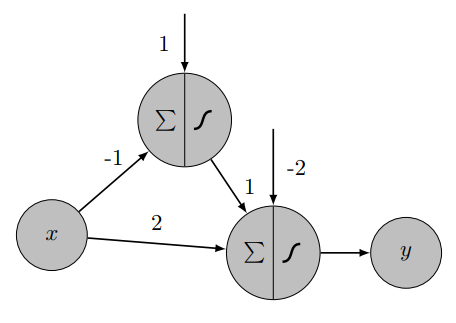
\includegraphics[width=.5\textwidth]{fig/2018-03-19-13-49-49.png}
	\caption{MLP with two logistic units} \label{fig:mlp}
\end{figure}

\begin{description}
	\item[a).]	Both neurons use the logistic activation function
	      $f(u)=\frac{1}{1+e^{-u}}$
	      The network has
	      a single input variable $x$ and one output variable $y$. Calculate the output of both
	      neurons and the error made by the MLP when applying a pattern with $x = 0$ and
	      target value $0.5$.
	\item[b).] Calculate the partial derivatives of the
	      square error $\frac{1}{2}(\hat{y} -y)^2$
	      with respect to the weights for the pattern used in task a).
\end{description}

\subsection{Forward-Backward-Pass}

{
	\centering
	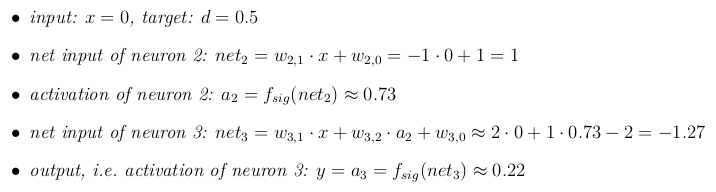
\includegraphics[width=.9\textwidth]{fig/2018-04-02-14-48-39.png} \\
	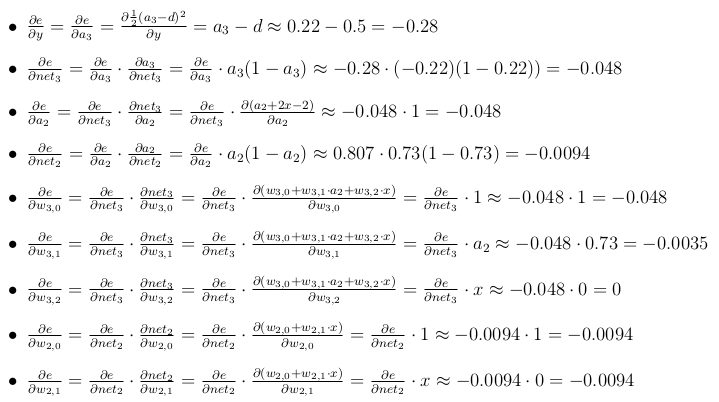
\includegraphics[width=.9\textwidth]{fig/2018-04-02-14-49-31.png}
}

% ----------------------------------------------------------------------------------------
\newpage 
\section{Multi-Layer Perceptron Architecture}

\begin{figure}[!htbp]
	\centering
	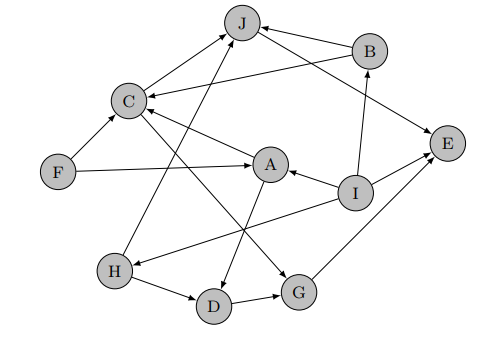
\includegraphics[width=.55\textwidth]{fig/2018-03-19-13-54-31.png}
	\caption{MLP with ten neurons} \label{fig:mlp2}
\end{figure}

Now, consider the network structure of a multi-layer perceptron with 10 neurons given in
fig~\ref{fig:mlp2}. Each circle denotes a neuron, the arrows denote connections between neurons.
\begin{description}
	\item[a).]  Which of the neurons are input neurons, which ones are output neurons?
	\item[b).] How many layers does this MLP have? Which neurons belong to which layer?
	\item[c).] Assume we are applying a pattern to the MLP. Give an order in which the neuron
	      activations $a_i$ can be calculated.
\end{description}

\subsection{Multi-Layer Perceptron Architecture}

\begin{center}
	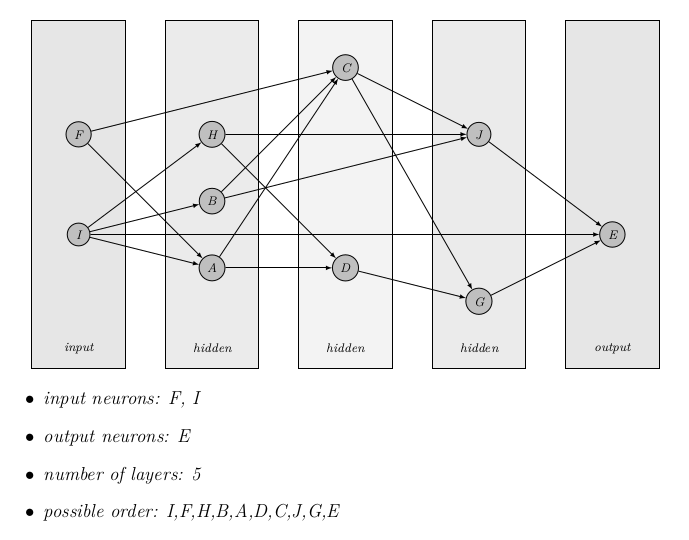
\includegraphics[width=.9\textwidth]{fig/2018-04-02-14-57-10.png}
\end{center}

% ----------------------------------------------------------------------------------------
\newpage
\section{Multi-Layer Perceptrons}

Which of the functions given by the plots in fig~\ref{fig:mlp3} can be implemented by multi-layer
perceptrons? The MLP should only contain neurons with logistic activation functions.
(Note: The weights of the networks must be finite numbers.)

\begin{figure}
	\centering

	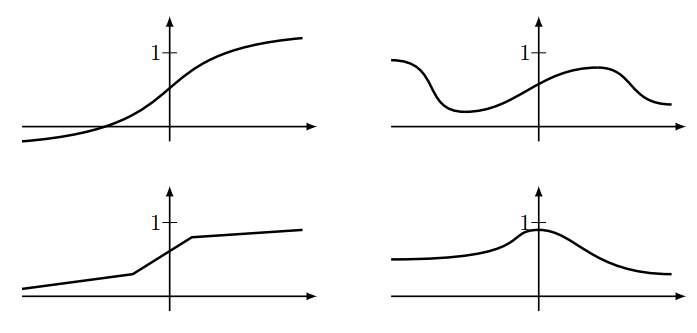
\includegraphics[width=.75\textwidth]{fig/2018-03-19-13-57-32.png}
	\caption{Functions to be realized by MLPs} \label{fig:mlp3}
\end{figure}

\subsection{Multi-Layer Perceptron}

\begin{itemize}
	\tightlist
	\item TL: no (since logistic function yields values between 0 and 1)
	\item TR: yes
	\item  BL: no (function must be differentiable)
	\item  BR: yes
\end{itemize}

% ----------------------------------------------------------------------------------------
\newpage 
\section{MLP and BackPropogation} \label{sec:3}

\begin{itemize}

	\item Download \textit{hw2.zip} from ftp(10.13.71.168), The code pass test under Python 2.7.14 and Python 3.6.3. Complete code surrounded by ``TODO'' in \textit{net.py} and \textit{opt.py}. For example,
	      \begin{verbatim}
###########################################################################
# TODO: Implement the affine forward pass. Store the result in out. You   #
# will need to reshape the input into rows.                               #
###########################################################################


###########################################################################
#                             END OF YOUR CODE                            #
###########################################################################
	\end{verbatim}
	\item Run \textit{python main\_check.py} and paste the settings (\eg random seed, loss function name) and the results to  your report.  Make sure your code pass gradient check, \eg, relative error between Numerical gradient and analytic gradient is small (\textit{e.g.} smaller than 1e-7). We use centered formula $\displaystyle \frac{\mathrm{d}f(x)}{\mathrm{d}x} \approx \frac{f(x+h)-f(x)}{h}$ to compute numerical gradient since it has an error on order of $O(h)$ and use relative error as metric.
	\item Run \textit{python main\_train.py} to train a model on generated fake data.
	\item {{Bonus(answer one of them is enough)}}: Do something extra surrounding the topics in this assignment, using the code you developed. For example, is there some other interesting question we could have asked? Is there any insightful visualization you can plot? For example, you can compare the convergence speed and performance of  linear regression and/or logistic regression and/or two-class softmax classification. You can select \textbf{some} samples (\textit{e.g.} 50 or 500) in cifar10 or use the dataset in {Problem~\ref{sec:4}} to do real case analysis and will MLP overfit on small subset on cifar10? If the generated fake data is imbalanced, what would happend and how to deal with it?  \textit{et. al.}
	\item You do not necessarily strictly use the framework provided by teacher assistant. You can use any language and framework and write from scratch.
	      Even tensorflow/pytorch with autograd is permitted, if you have time.
	      Just make sure implement MLP by yourself and then do similar experiments, \textit{i.e.}, do not use any function like MLP or LinearRegression.
	\item Finally, upload to ftp(10.13.72.84) before the deadline(Sunday, April 1, 23:59:59).
\end{itemize}

\subsection{MLP and BackPropogation} 

After filling the code and running the \textit{main\_check.py}, I get the results as following. There are other parameters settings and results, so we just need to make sure relative errors smaller than 1e-7. 

\begin{verbatim}
	loss use softmax
	----------------
	Testing test-time forward pass
	scores are [[-1.372  0.972]
	 [-0.876  1.132]
	 [-0.38   1.292]]
	----------------
	Testing training loss
	loss is 1.4685851981586016
	W1 relative error: 4.65e-11
	W2 relative error: 1.27e-11
	b1 relative error: 5.55e-12
	b2 relative error: 1.19e-11	
\end{verbatim}
I set the hyper-parameters as
\begin{verbatim}
Left fig: 
N, D, H, C = small_data['X_train'].shape[0], 2, 10, 2
loss = 'softmax'

Right fig:
N, D, H, C = small_data['X_train'].shape[0], 2, 10, 1
loss = 'mse'
\end{verbatim}

\begin{center}
	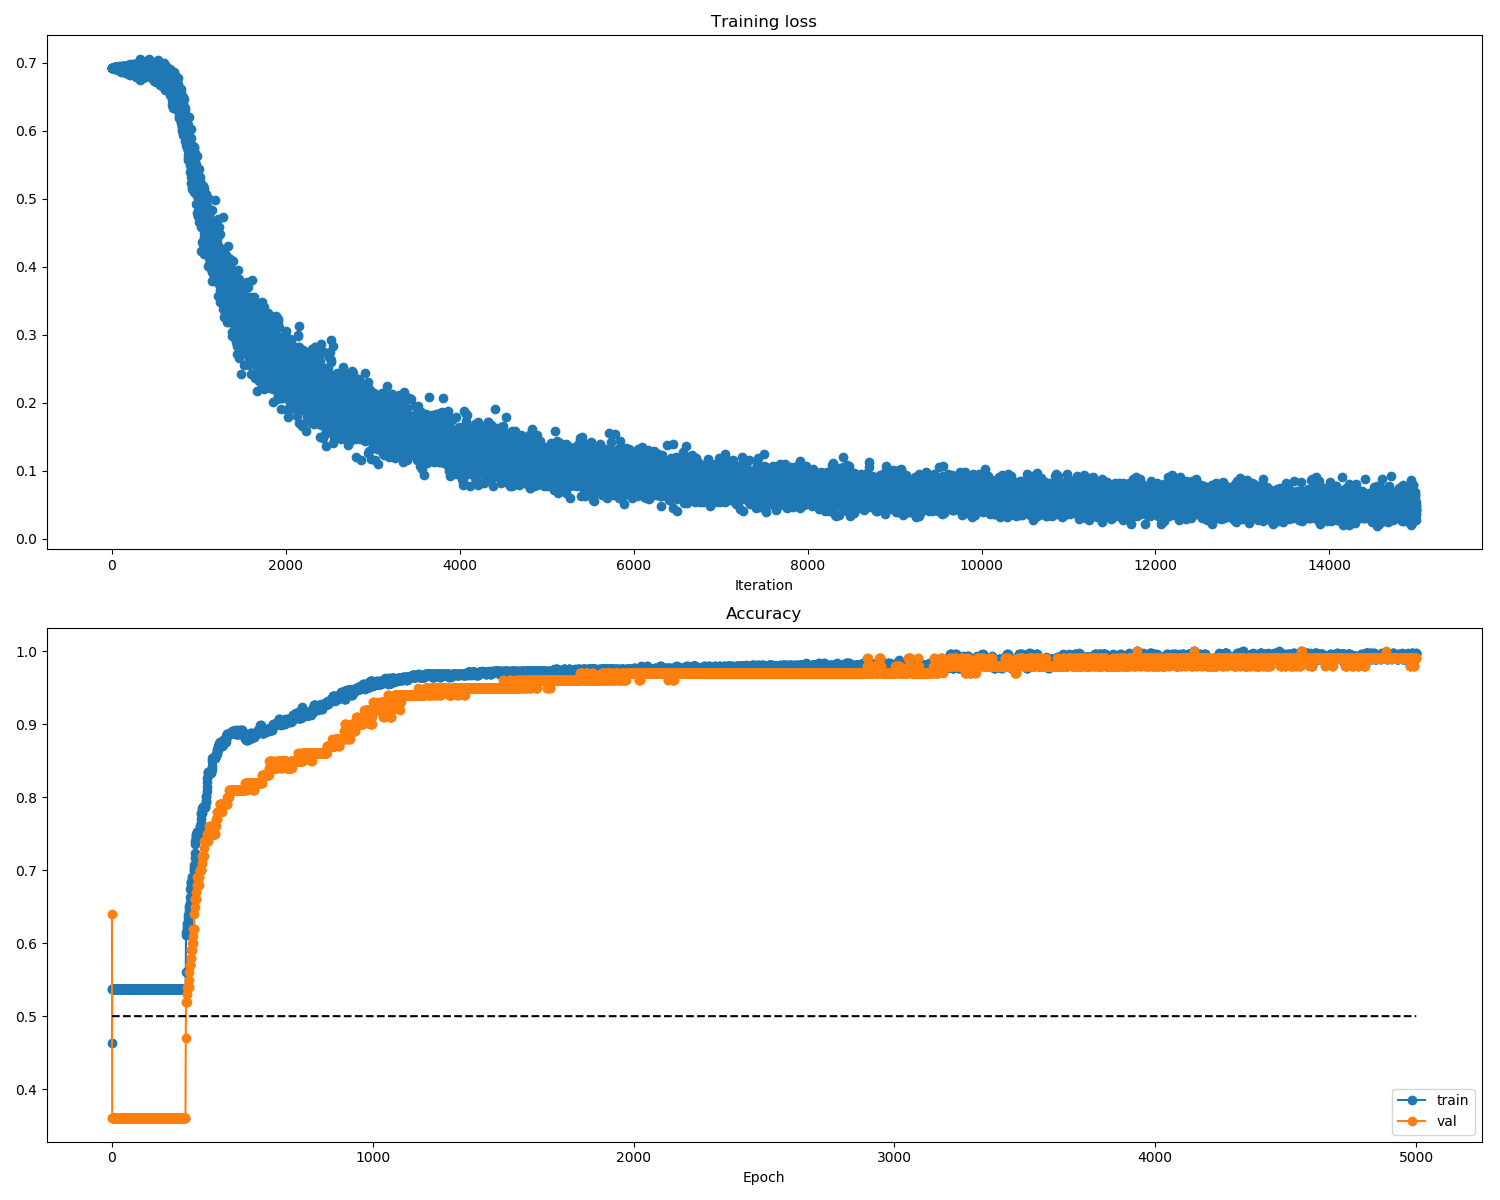
\includegraphics[width=.49\textwidth]{fig/2018-04-02-15-16-43.png}
	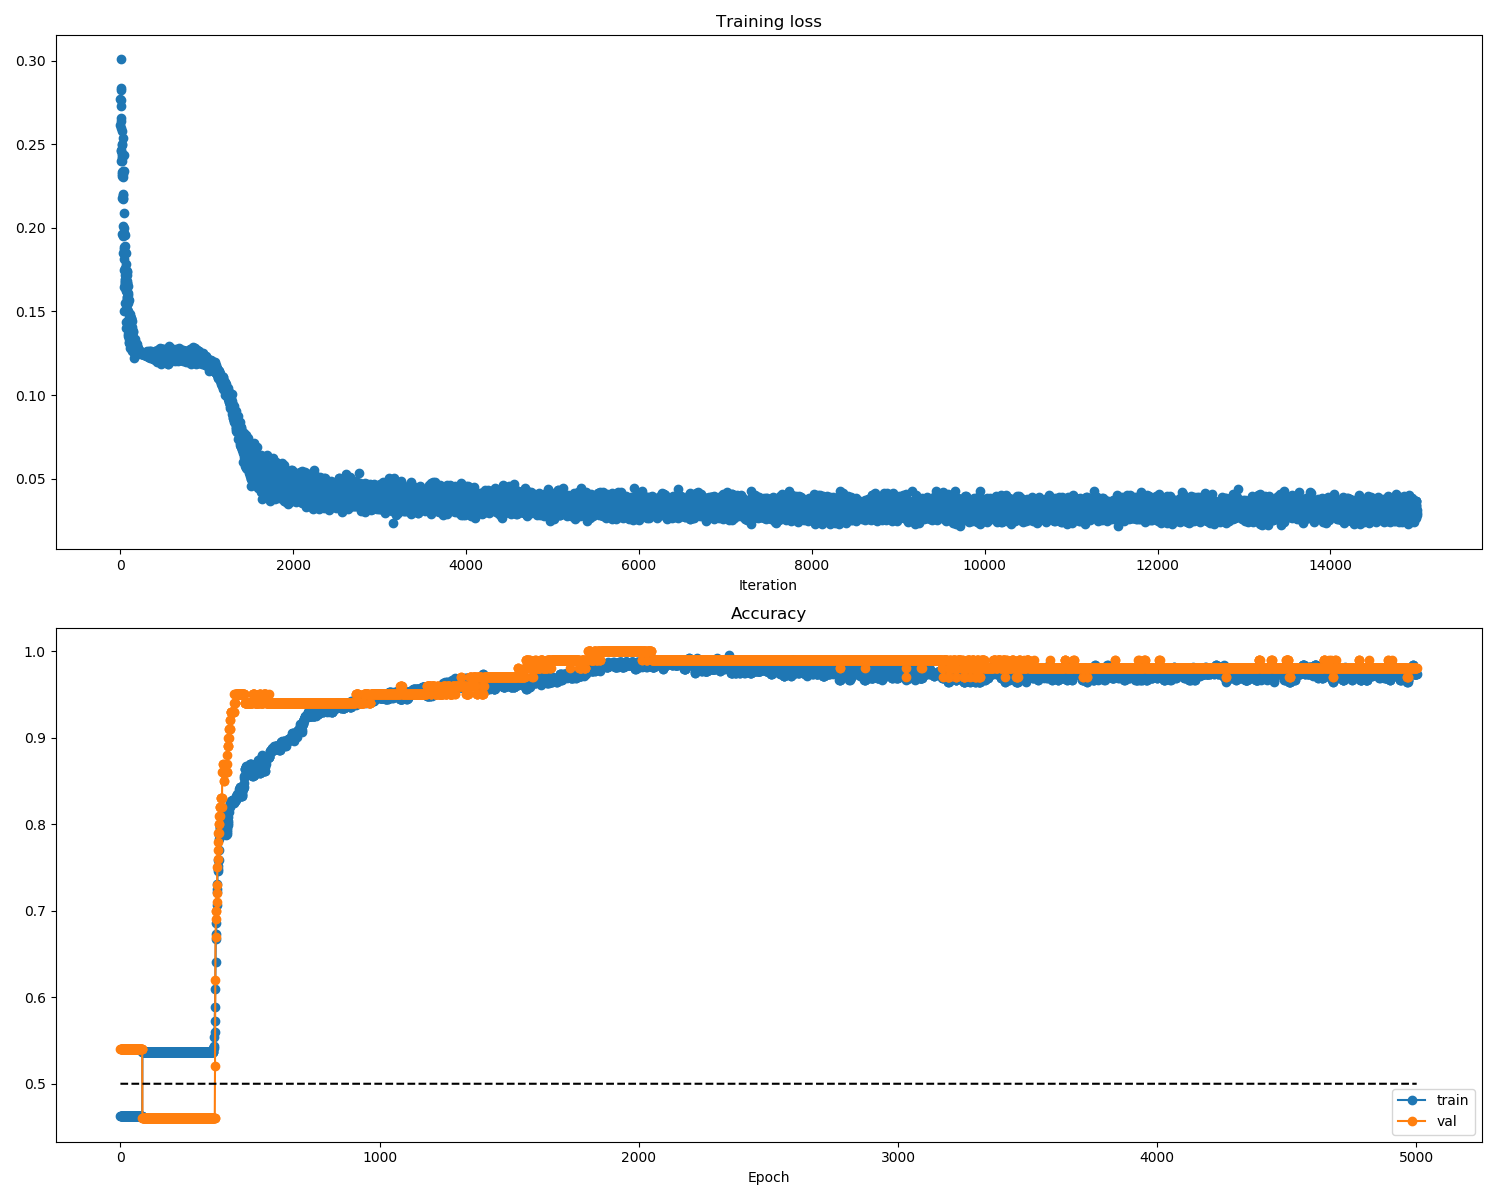
\includegraphics[width=.49\textwidth]{fig/2018-04-02-15-15-07.png} 
\end{center}

% ----------------------------------------------------------------------------------------
\newpage 
\section{Predict House Prices} \label{sec:4}
Given 79 explanatory variables describing (almost) every aspect of residential homes, such as the size  and the location of the house, please predict the final price of each home.

\begin{itemize}
	\item  Download \textit{hw2.zip} from ftp(10.13.71.168). The dataset is cleaned to become simple train/val format. You can try to modify the process of data clean.
	\item Make sure implement the {linear} regression model by yourself and do not use {{`LinearRegression' in `sklearn'}}.  Linear regression optimized by sgd is similar to MLP, which have been implemented in {Problem~\ref{sec:3}}. You can also use closed form solution for linear regression with/without $l_2$ regularization. 

	\textit{hint:} $l_2$ regularization is equivalent to pertubation, makes sure the inverse of matrix exits.

	\item {{Bonus(answer one of them is enough)}}: Do something extra surrounding the topics in this assignment, using the code you developed. For example, try lasso regression and/or huber loss and/or learning rate decay and/or select best model by cross validation. What would happen if the x and y do not subtract mean? If you implement linear  regression by  closed-form formulation and sgd, you can compare them on speed and performance. \textit{et. al.} 

	\item You do not necessarily strictly use the framework provided by teacher assistant. You can use any language and write from scratch. Just make sure implement regression model by yourself and then do similar experiments.
	\item Finally, upload to ftp(10.13.72.84) before the deadline(Sunday, April 1, 24:00:00).
\end{itemize}

\subsection{Predict House Prices}

r2\_socre: 0.86\~0.88

\end{document}

